\section{Phương pháp luận và Khung giải pháp đề xuất}
Để giải quyết hiệu quả các thách thức kép về sự mất cân bằng dữ liệu cực đoan và định kiến thuật toán đơn lẻ trong NIDS, chúng tôi đề xuất một khung giải pháp được tối ưu hóa toàn diện. Phần này trình bày chi tiết quy trình tiền xử lý dữ liệu, chiến lược lấy mẫu cân bằng nâng cao và nền tảng toán học của Kiến trúc Ensemble lai mới của chúng tôi.

\subsection{Tiền xử lý dữ liệu \& Kỹ thuật đặc trưng}
Bộ dữ liệu CICIDS2017 có đặc điểm là số chiều lớn (hơn 78 đặc trưng thô), phương sai đáng kể và sự tồn tại của các giá trị bị thiếu (NaN) hoặc vô hạn do lỗi luồng gói tin gây ra. Trước khi đưa vào thuật toán, một quy trình tiền xử lý nghiêm ngặt sẽ được thực hiện.

\subsubsection{Làm sạch dữ liệu và gán nhãn} 
Các bản ghi chứa giá trị \texttt{NaN} hoặc \texttt{Infinity} được tách biệt một cách hệ thống. Với khối lượng lớn của lớp đa số, các mẫu có phân phối thống kê bị hỏng không thể phục hồi sẽ bị loại bỏ thay vì được gán nhãn bù để ngăn chặn việc đưa vào nhiễu tổng hợp. Đối với các đặc trưng luồng liên tục (ví dụ: \textit{Flow Duration}, \textit{Packet Length Variance}), kỹ thuật gán nhãn thống kê mạnh mẽ bằng các giá trị trung vị theo nhóm lớp tấn công được áp dụng khi cần thiết để bảo toàn phân phối cơ bản.

\subsubsection{Chuẩn hóa và Co giãn dữ liệu} 
Sự khác biệt về quy mô của các phép đo lưu lượng mạng (ví dụ: số byte so với thời gian micro giây) vốn dĩ gây ra định kiến cho các thuật toán dựa trên khoảng cách hoặc giảm gradient, đồng thời cũng chịu ảnh hưởng bởi các giá trị ngoại lai (outliers). Để giảm thiểu tác động của các giá trị ngoại lai, chúng tôi áp dụng Robust Scaling thay vì Min-Max hay chuẩn hóa tiêu chuẩn. Các biến liên tục $x_i$ được co giãn bằng cách sử dụng giá trị trung vị $\tilde{x}$ và Khoảng tứ phân vị (Interquartile Range - IQR):
\begin{equation}
x_{norm} = \frac{x_i - \tilde{x}}{\text{IQR}(X)}
\end{equation}
trong đó $X$ đại diện cho không gian vectơ của đặc trưng cụ thể.

\begin{figure}[htbp]
\centering
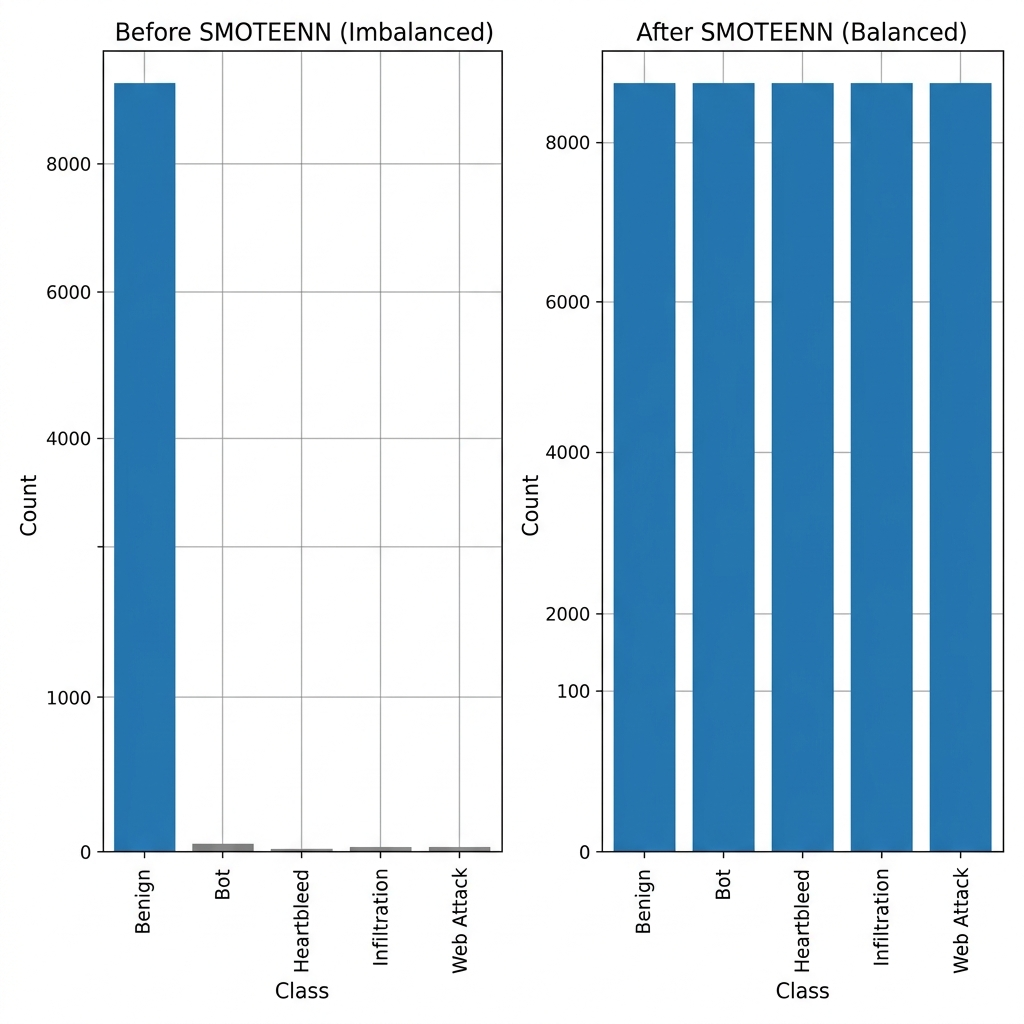
\includegraphics[width=\columnwidth]{figures/dataset_balance.png}
\caption{Phân phối các lớp của bộ dữ liệu CICIDS2017 trước và sau khi áp dụng kỹ thuật lấy mẫu lại SMOTEENN.}
\label{fig:dataset_balance}
\end{figure}

\subsubsection{Chiến lược lấy mẫu cân bằng với SMOTEENN}
Để khắc phục tình trạng thiểu số cực đoan của các cuộc tấn công cụ thể (chẳng hạn như Heartbleed và Infiltration, chiếm $<0,01\%$ bộ dữ liệu), chúng tôi triển khai chiến lược lấy mẫu lai SMOTEENN (SMOTE kết hợp với Edited Nearest Neighbors). Trong khi kỹ thuật SMOTE (Synthetic Minority Over-sampling Technique) tiêu chuẩn \cite{chawla2002smote} tổng hợp hiệu quả các phiên bản thiểu số mới, nó thực hiện nội suy tuyến tính giữa các mẫu thiểu số, thường tạo ra các vectơ đặc trưng vượt qua ranh giới quyết định sang vùng của lớp lành tính trong không gian đa chiều, từ đó gây ra nhiễu.

Để giải quyết vấn đề này, thuật toán SMOTEENN \cite{batista2004study} được sử dụng như một cơ chế làm sạch dữ liệu nâng cao. Tuy nhiên, việc áp dụng trực tiếp thuật toán ENN (vốn có độ phức tạp $O(N^2)$ để tính toán khoảng cách) trên toàn bộ lớp đa số (hơn 2 triệu mẫu của CICIDS2017) là không khả thi về mặt thời gian và tài nguyên tính toán. Do đó, chúng tôi đề xuất một chiến lược tiền xử lý bổ sung: đầu tiên, kỹ thuật Random Under-sampling (RUS) được áp dụng để giảm ngẫu nhiên kích thước của lớp đa số xuống mức cân bằng tương đối với lớp thiểu số. Bước thu gọn này giúp loại bỏ một lượng lớn các mẫu dư thừa ở xa ranh giới quyết định.

Sau khi lớp đa số đã được thu gọn, SMOTEENN được áp dụng. Nó trước tiên sử dụng SMOTE để tổng hợp thêm các mẫu thiểu số, sau đó Edited Nearest Neighbors (ENN) \cite{wilson1972asymptotic} đánh giá vùng lân cận của mỗi mẫu bằng quy tắc $k$-lân cận gần nhất để loại bỏ các mẫu nhiễu nằm sai lớp. Sự kết hợp tinh tế giữa RUS và SMOTEENN không chỉ giảm triệt để thời gian tính toán từ nhiều ngày xuống còn vài phút, mà còn xây dựng lại một cách mạnh mẽ một không gian vectơ huấn luyện $S_{train}$ được căn chỉnh, không có nhiễu và ranh giới quyết định duy trì được sự sắc nét tối đa.

% ==========================================
% THUẬT TOÁN 1: Tiền xử lý và SMOTEENN
% ==========================================
\begin{algorithm}[hbt!]
\SetAlgoLined
\KwIn{Bộ dữ liệu lưu lượng mạng thô $\mathcal{D} = \{(x_1, y_1), \dots, (x_N, y_N)\}$}
\KwOut{Bộ dữ liệu đã được làm sạch, co giãn và cân bằng $\mathcal{D}_{bal}$}

\tcc{Bước 1: Làm sạch dữ liệu}
$\mathcal{D}_{clean} \leftarrow \emptyset$\;
\ForEach{$(x_i, y_i) \in \mathcal{D}$}{
    \If{$x_i \notin \{\text{NaN}, \text{Inf}\}$ \textbf{và} $(x_i, y_i) \notin \mathcal{D}_{clean}$}{
        $\mathcal{D}_{clean} \leftarrow \mathcal{D}_{clean} \cup \{(x_i, y_i)\}$\;
    }
}

\tcc{Bước 2: Co giãn đặc trưng}
Giả sử $X \subset \mathcal{D}_{clean}$ là không gian đặc trưng\;
Tính trung vị $\tilde{x}$ và Khoảng tứ phân vị (IQR) cho $X$\;
\ForEach{$x_i \in X$}{
    $x'_i \leftarrow \frac{x_i - \tilde{x}}{\text{IQR}}$ \tcp*{Áp dụng Robust Scaler}
}
$\mathcal{D}_{scaled} \leftarrow (X', Y_{clean})$\;

\tcc{Bước 3: Xử lý mất cân bằng lớp}
Chia $\mathcal{D}_{scaled}$ thành lớp đa số $\mathcal{S}_{maj}$ và các lớp thiểu số $\mathcal{S}_{min}$\;

\tcc{Bước 3.1: Tiền giảm mẫu bằng RUS}
Giảm ngẫu nhiên $\mathcal{S}_{maj}$ xuống kích thước tương đương lớp thiểu số để tạo $\mathcal{S}'_{maj}$\;

\tcc{Bước 3.2: Sinh dữ liệu SMOTE}
$\mathcal{S}_{syn} \leftarrow \emptyset$\;
\ForEach{$x \in \mathcal{S}_{min}$}{
    Tìm $k$-lân cận gần nhất $N_k(x)$\;
    Lấy mẫu lân cận $x_{nn} \sim $ của $N_k(x)$\;
    Tạo $x_{new} \leftarrow x + \delta \cdot (x_{nn} - x)$ với $\delta \sim U(0,1)$\;
    $\mathcal{S}_{syn} \leftarrow \mathcal{S}_{syn} \cup \{x_{new}\}$\;
}
$\mathcal{D}_{SMOTE} \leftarrow \mathcal{S}'_{maj} \cup \mathcal{S}_{min} \cup \mathcal{S}_{syn}$\;

\tcc{Bước 3.3: Làm sạch ENN}
\ForEach{$(x_i, y_i) \in \mathcal{D}_{SMOTE}$}{
    Tìm 3-lân cận gần nhất $N_3(x_i)$\;
    \If{lớp đa số của $N_3(x_i) \neq y_i$}{
        $\mathcal{D}_{SMOTE} \leftarrow \mathcal{D}_{SMOTE} \setminus \{(x_i, y_i)\}$ \tcp*{Loại bỏ mẫu nhiễu}
    }
}
$\mathcal{D}_{bal} \leftarrow \mathcal{D}_{SMOTE}$\;

\Return{$\mathcal{D}_{bal}$}
\caption{Tiền xử lý dữ liệu mạnh mẽ và cân bằng bằng SMOTEENN}
\label{algo:preprocessing}
\end{algorithm}

\subsection{Kiến trúc Ensemble lai}
Khi không gian đa chiều đã được cân bằng, dữ liệu sẽ được đưa vào Kiến trúc Ensemble lai của chúng tôi. Chúng tôi sử dụng một cách chiến lược một tập hợp đa dạng các bộ phân loại cơ sở (base learners) có khả năng nắm bắt các cấu trúc dạng bảng không đồng nhất và các mối quan hệ phi tuyến tính sâu sắc, được tổng hợp bởi một bộ phân loại meta (meta-classifier) đơn giản và dễ giải thích.

\subsubsection{Các bộ phân loại cơ sở: XGBoost, LightGBM và Random Forest}
Các thuật toán dựa trên cây đã được chứng minh là vượt trội trong việc trích xuất các cấu trúc tiềm ẩn từ không gian đặc trưng dạng bảng không đồng nhất. Chúng tôi kết hợp một cách chiến lược hai phương pháp bổ trợ cho nhau—tăng cường gradient (boosting) và bagging—để tối đa hóa sự đa dạng của tập hợp.
\begin{itemize}
    \item \textbf{XGBoost}: Hoạt động bằng cách thêm tuần tự các cây quyết định để sửa lỗi dư (residual errors) của các cây trước đó \cite{friedman2001greedy, chen2016xgboost}. Giả sử dự đoán tại bước $t$ là $\hat{y}_i^{(t)} = \hat{y}_i^{(t-1)} + f_t(x_i)$. XGBoost giảm thiểu hàm mục tiêu:
    \begin{equation}
        Obj^{(t)} = \sum_{i=1}^{n} l\left(y_i, \hat{y}_i^{(t-1)} + f_t(x_i)\right) + \Omega(f_t)
    \end{equation}
    trong đó $l$ là hàm mất mát lồi có đạo hàm, và $\Omega$ phạt độ phức tạp của mô hình để giảm thiểu phương sai.
    \item \textbf{LightGBM}: Giới thiệu kỹ thuật \textit{Gradient-based One-Side Sampling} (GOSS) và \textit{Exclusive Feature Bundling} (EFB) \cite{ke2017lightgbm}. Các cơ chế này cho phép LightGBM xử lý các bộ dữ liệu khổng lồ với tốc độ cao trong khi vẫn giữ được ranh giới quyết định chặt chẽ từ các phiên bản có gradient lớn hơn.
    \item \textbf{Random Forest}: Một tập hợp các cây quyết định được huấn luyện trên các mẫu bootstrap của dữ liệu, sử dụng các tập con đặc trưng ngẫu nhiên tại mỗi điểm chia \cite{breiman2001random}. Bằng cách tổng hợp các dự đoán từ $T$ cây độc lập, Random Forest giảm phương sai thông qua việc tổng hợp bootstrap song song:
    \begin{equation}
        \hat{y}_{RF}(x) = \frac{1}{T} \sum_{t=1}^{T} h_t(x)
    \end{equation}
    trong đó $h_t$ đại diện cho từng cây quyết định riêng lẻ. Phương pháp bagging này cung cấp sự đa dạng về thuật toán bổ trợ cho phương pháp boosting tuần tự của XGBoost và LightGBM.
\end{itemize}
Ba bộ phân loại cơ sở đa dạng này tạo ra các dự đoán xác suất $P_{XGB}(y|x)$, $P_{LGBM}(y|x)$, và $P_{RF}(y|x)$ được hiệu chuẩn cao.

\subsubsection{Bộ phân loại Meta: Logistic Regression}
Để đưa ra kết quả phân loại cuối cùng, chúng tôi sử dụng Hồi quy Logistic (Logistic Regression) làm bộ phân loại meta trong cấu hình Stacking. Các đầu ra xác suất từ các bộ phân loại cơ sở được nối lại để tạo thành một vectơ đặc trưng meta mới $Z_i = [P_{XGB}(y|x_i), P_{LGBM}(y|x_i), P_{RF}(y|x_i)]$.

Hồi quy Logistic học một tổ hợp tuyến tính của các dự đoán chuyên gia này bằng cách tối ưu hóa một tập hợp các trọng số $W$, áp dụng hàm sigmoid cho đầu ra phân loại nhị phân:
\begin{equation}
    \hat{Y} = \sigma(W \cdot Z_i + b) = \frac{1}{1 + e^{-(W \cdot Z_i + b)}}
\end{equation}

Bằng cách sử dụng một bộ phân loại meta tuyến tính trên các gradient dự đoán của một cơ sở ensemble đa dạng, khung giải pháp sẽ học cách tin tưởng các bộ phân loại cơ sở cụ thể cho các dấu hiệu tấn công khác nhau một cách linh hoạt mà không gặp rủi ro quá tải (overfitting) nghiêm trọng ở mức độ meta. Kiến trúc stacking phân cấp này kết hợp hiệu quả các thế mạnh bổ trợ của phương pháp boosting và bagging, giúp giảm thiểu đáng kể tỷ lệ Cảnh báo sai.

% ==========================================
% THUẬT TOÁN 2: Kiến trúc Ensemble lai
% ==========================================
\begin{algorithm}[hbt!]
\SetAlgoLined
\KwIn{Bộ dữ liệu huấn luyện đã cân bằng $\mathcal{D}_{bal} = (X_{train}, Y_{train})$}
\KwOut{Mô hình Ensemble lai đã tối ưu hóa $\mathcal{E}$}

\tcc{Bước 1: Khởi tạo các bộ phân loại cơ sở}
$M_1 \leftarrow$ XGBoost Classifier\;
$M_2 \leftarrow$ LightGBM Classifier\;
$M_3 \leftarrow$ Random Forest Classifier\;
$M_{base} \leftarrow \{M_1, M_2, M_3\}$\;

\tcc{Bước 2: Tạo dự đoán Out-of-Fold (Stacking)}
$\mathcal{D}_{meta} \leftarrow \emptyset$\;
\ForEach{$M_i \in M_{base}$}{
    Huấn luyện $M_i$ trên $(X_{train}, Y_{train})$ sử dụng $k$-fold cross-validation\;
    Trích xuất xác suất dự đoán $P_i(y|x)$ cho $X_{train}$\;
}

\tcc{Bước 3: Xây dựng bộ dữ liệu Meta}
\ForEach{$x_j \in X_{train}$}{
    $P^{(j)} \leftarrow \left[ P_1(y|x_j), P_2(y|x_j), P_3(y|x_j) \right]$\;
    $\mathcal{D}_{meta} \leftarrow \mathcal{D}_{meta} \cup \{(P^{(j)}, y_j)\}$\;
}

\tcc{Bước 4: Huấn luyện bộ phân loại Meta}
Khởi tạo bộ phân loại Meta $M_{meta}$ (Logistic Regression)\;
Huấn luyện $M_{meta}$ trên $\mathcal{D}_{meta}$\;

\tcc{Bước 5: Thiết lập mô hình Ensemble cuối cùng}
Xác định hàm dự đoán ensemble $\hat{y}$ cho một đầu vào mới $x_{test}$:\;
$\hat{y}(x_{test}) = M_{meta} \left( [M_1(x_{test}), M_2(x_{test}), M_3(x_{test})] \right)$\;
$\mathcal{E} \leftarrow \{M_{base}, M_{meta}, \hat{y}\}$\;

\Return{$\mathcal{E}$}
\caption{Huấn luyện mô hình Ensemble lai (XGBoost, LightGBM, Random Forest)}
\label{algo:ensemble}
\end{algorithm}

\subsection{Chưng cất tri thức cho triển khai tại biên}
Mặc dù Kiến trúc Ensemble lai đạt được độ chính xác hiện đại, sự phụ thuộc vào ba mô hình dựa trên cây đa dạng gây ra chi phí tính toán lớn, có khả năng hạn chế khả năng triển khai trên các thiết bị Biên và Internet Vạn vật (IoT) hạn chế về tài nguyên. Để thu hẹp khoảng cách giữa độ chính xác cao và độ trễ suy luận thấp, chúng tôi đề xuất mở rộng bằng kỹ thuật Chưng cất Tri thức (Knowledge Distillation - KD).

Chưng cất Tri thức là một cơ chế nén mô hình, trong đó một mô hình "Học sinh" (Student) nhỏ và hiệu quả cao được huấn luyện để mô phỏng hành vi của một mô hình "Giáo viên" (Teacher) lớn và phức tạp \cite{hinton2015distilling} (là mô hình Ensemble lai $\mathcal{E}$ của chúng tôi). Trong kỹ thuật KD truyền thống cho các mạng thần kinh, Student học từ các "nhãn mềm" (soft labels - xác suất các lớp) do Teacher tạo ra.

Trong khung giải pháp của mình, chúng tôi sử dụng một Cây Quyết định nhẹ (với độ sâu tối đa bị hạn chế) làm mô hình Student ($M_{student}$). Mô hình Teacher thực hiện suy luận trên tập huấn luyện cân bằng $X_{train}$ để tạo ra một tập hợp các nhãn mục tiêu có độ chính xác cao $\hat{Y}_{teacher}$. Sau đó, Student được huấn luyện để giảm thiểu rủi ro thực nghiệm so với các dự đoán của Teacher thay vì các nhãn gốc:
\begin{equation}
    \min_{\theta_{student}} \sum_{i=1}^{N} \mathcal{L}\left( M_{student}(x_i; \theta_{student}), \hat{Y}_{teacher}^{(i)} \right)
\end{equation}

Bằng cách trích xuất các ranh giới quyết định phức tạp mà mô hình tập hợp khổng lồ đã học được và đưa chúng vào một cấu trúc cây nông duy nhất, mô hình Student thừa hưởng một phần đáng kể khả năng tổng quát hóa của Teacher. Quá trình này giúp giảm đáng kể số lượng các phép toán dấu phẩy động cần thiết cho mỗi lần phân loại, tối ưu hóa Hệ thống Phát hiện Xâm nhập cho các môi trường mạng thời gian thực, thông lượng cao với yêu cầu độ trễ dưới một phần nghìn giây. Quy trình chưng cất rõ ràng được trình bày trong Thuật toán~\ref{algo:kd}.

\begin{algorithm}[ht]
\DontPrintSemicolon
\SetAlgoLined
\KwIn{Tập đặc trưng cân bằng $X_{train}$, Nhãn gốc $Y_{train}$, Mô hình Teacher đã huấn luyện $\mathcal{E}$, Độ sâu tối đa của cây Student $d$}
\KwOut{Mô hình Student đã tối ưu hóa để triển khai Edge $M_{student}$}
\tcp{Bước 1: Tạo nhãn Mềm/Cứng bằng mô hình Teacher}
$\hat{Y}_{teacher} \leftarrow \emptyset$ \;
\For{$i = 1 \dots N$}{
    $p_i \leftarrow \mathcal{E}.predict\_proba(x_i)$ \tcp*{Lấy xác suất đầu ra}
    $\hat{y}^{(i)}_{teacher} \leftarrow \arg\max(p_i)$ \tcp*{Chuyển sang nhãn chính xác}
    $\hat{Y}_{teacher} \leftarrow \hat{Y}_{teacher} \cup \{\hat{y}^{(i)}_{teacher}\}$ \;
}
\tcp{Bước 2: Huấn luyện mô hình Student nhẹ}
Khởi tạo Cây quyết định $M_{student}$ với tham số max\_depth=$d$ \;
$M_{student}.fit(X_{train}, \hat{Y}_{teacher})$ \tcp*{Học các ranh giới của Teacher}
\tcp{Bước 3: Đánh giá dấu ấn triển khai}
Tính toán $Size(M_{student})$ so với $Size(\mathcal{E})$ \tcp*{Kiểm tra mức độ nén bộ nhớ}
Tính toán $Latency(M_{student})$ so với $Latency(\mathcal{E})$ \tcp*{Kiểm tra mức độ tăng tốc}
\Return $M_{student}$ \;
\caption{Chưng cất Tri thức Giáo viên-Học sinh để triển khai tại biên}
\label{algo:kd}
\end{algorithm}
